%%%%%%%%%%%%%%%%%%%%%%%%%%%%%%%%%%%%%%%%%
% Original author:
% Linux and Unix Users Group at Virginia Tech Wiki
% (https://vtluug.org/wiki/Example_LaTeX_chem_lab_report)
% Modified by: Hector F. Jimenez S, for the Digital Electronics Laboratory.
% License:
% CC BY-NC-SA 3.0 
%%%%%%%%%%%%%%%%%%%%%%%%%%%%%%%%%%%%%%%%%
%----------------------------------------
%	PACKAGES AND DOCUMENT CONFIGURATIONS
%---------------------------------------
\documentclass[paper=a4, fontsize=12pt]{article} 		% A4 paper and 11pt font size
\usepackage[T1]{fontenc} 								% Use 8-bit encoding that has 256 glyphs
%\usepackage{fourier}		 							% Use the Adobe Utopia font for the document 
\usepackage[spanish,english]{babel}						% Spanish Language, templates uses some sections in english.
\selectlanguage{spanish}								% main language.
\usepackage{subfig}
\usepackage{multirow}
\PassOptionsToPackage{spanish}{babel}
\renewcommand{\figurename}{Figura}						% Force rename of figure.
\renewcommand{\figurename}{Fig.}
\usepackage[figurename=Fig.]{caption}
\usepackage[utf8]{inputenc}								% tildes for spanish language.
\usepackage{amsmath,amsfonts,amsthm} 					% Math packages.
\usepackage{minted}										% For syntax highlighting.
	    \renewcommand\listingscaption{Código}			%rename the source code minted !
\usepackage{float}										% Image will be in the same place as you want.!!! x-/
\usepackage{sectsty} 									% Allows customizing section commands
\allsectionsfont{\centering \normalfont\scshape}	   	% Make all sections centered, the default font and small caps
\usepackage{hyperref}
\hypersetup{											%Setups the false color and borders.
    colorlinks=false,
    pdfborder={0 0 0},
}
\newcommand\fnurl[2]{%									% set a simple and quick footnote command and include url.
\href{#2}{#1}\footnote{\url{#2}}%	
}
\usepackage{graphicx}									% Import easyly images.
\graphicspath{ {./images/} }							% Where to look for the images.
\DeclareGraphicsExtensions{.pdf,.png,.jpg}				% Graphics Extension to be used
\usepackage[notes,backend=biber]{biblatex-chicago}		% Bibliography and references.
\bibliography{biblio}									% bibliography filename.
\usepackage{fancyhdr} 									% Custom headers and footers
\pagestyle{fancyplain} 									% Makes all pages in the document conform to the custom headers and footers
\fancyhead{} 											% No page header
\fancyfoot[L]{} 										% Empty left footer
\fancyfoot[C]{} 										% Empty center footer
\fancyfoot[R]{\thepage} 								% Page numbering for right footer
\renewcommand{\headrulewidth}{0pt} 						% Remove header underlines
\renewcommand{\footrulewidth}{0pt} 						% Remove footer underlines
\setlength{\headheight}{13.6pt} 					    % Customize the height of the header
\numberwithin{equation}{section}						% Number equations within sections (i.e. 1.1, 1.2, 2.1, 2.2 instead of 1, 2, 3, 4)
%\numberwithin{figure}{section} 						% Number figures within sections (i.e. 1.1, 1.2, 2.1, 2.2 instead of 1, 2)
\numberwithin{table}{section} 							% Number tables within sections (i.e. 1.1, 1.2, 2.1, 2.2 instead of 1, 2, 3, 4)
\setlength\parindent{0pt} 								% Removes all indentation from paragraphs
\newcommand{\horrule}[1]{\rule{\linewidth}{#1}} 		% Create horizontal rule command with 1 argument of height
\usepackage{listings}% http://ctan.org/pkg/listings
\usepackage{multicol}
\usepackage{caption}
\usepackage{subfig}
\renewcommand{\lstlistingname}{Código}	
\title{Sistemas Operativos I\\ 
\horrule{0.5pt} \\[0.4cm] 								% Thin top horizontal rule	Title rule
\textit{Taller 4: Caso de estudio del sistema operativo MSDOS3.11, exploración superficial}
\horrule{1pt} \\[0.5cm] 			
} 			

\author{												
Héctor F. \textsc{Jiménez Saldarriaga.}\\				% Authors begin.
\texttt{hfjimenez@utp.edu.co} \\						
\texttt{PGP KEY ID: 0xB05AD7B8}
} 
% End of  Author name
\date{}    						                       % Date for the report, this will hide the \today.

\begin{document}
\maketitle                      			           % Insert the title, author and date
\begin{center}
\begin{tabular}{l r}								   % two column to
Fecha de Entrega: & Marzo, 2018 \\				   % Ramiro's Details.
Profesor: & Cesar Manuel Castillo Rodriguez
\end{tabular}
\end{center}
%%%%%%%%%%%	
% Let's start the document.
%%%%%%%%%%%	
\section{Objetivos}
\begin{itemize}
	\item Historia
	\item Realizar el proceso de instalación del sistema operativo	
    \item Identificar el manejo de Archivos, Shell
    \item Estructura del Sistema Operativo
    \item Clasificación del Sistema Operativo
	\item Instalación Software (Capturas de Pantalla)
\end{itemize}
\section{Historia}
La versión de Windows 3.11 fue liberada al publico a nivel comercial en en Noviembre 8, de 1993. No agrego muchas caracteristicas o mejoras, pero su mas sustancial mejora fue agregar drivers de vídeos y mejorar los protocolos de comunicacion pensadas en redes LAN, se piensa que la mayoría de los bugs corregidos de la versión predecesora (\textit{Windows3.0}) en la parte gráfica. Afortunadamente para ese entonces era fácil hacer el upgrade dado que era gratis si contabas con algunas versión de windows previa como fue nuestro caso.

Mas cambios sobre esta versión puede ser encontradas en \fnurl{Classic url}{https://classicreload.com/win3x-windows-311.html}
\section{Proceso de instalación MSDOS 3.11}
Para poder instalar windows 3.11 lo que nosotros hacemos es utilizar una versión previamente instalada de Windows MSDOS6.22, sobre esta instalación realizaremos un upgrade, al insertar el disquete en la unidad \textbf{\textit{A:}} lo que deberemos ejecutar es el setup.exe entregándonos la siguiente imagen con los pasos de instalación a seguir : 

\begin{figure}[H]
 	\centering
   	\subfloat[Actualización del sistema operativos MSDOS6.22, Setup de Windows3.11]{\label{fig:install}{
   		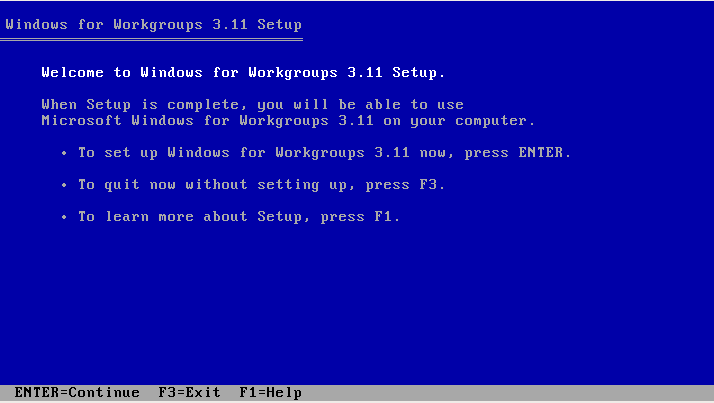
\includegraphics[scale=0.4]{img/1.png}}}
\end{figure}
Al seguir el proceso de instalación guiado es posible observar que es bastante simple realizarlo, ademas que contamos con la suerte de que no existen problemas en el proceso de instalación como disquetes ilegibles o errores en los archivos y su integridad. 
Seguidamente presionamos enter y ahora si a continuar con el proceso de instalación como se ve en las figuras.

\begin{figure}[H]
 	\centering
	\subfloat[Paso Inicial de Configuración Windows3.11 setup]{\label{fig:sugerencia}{
   		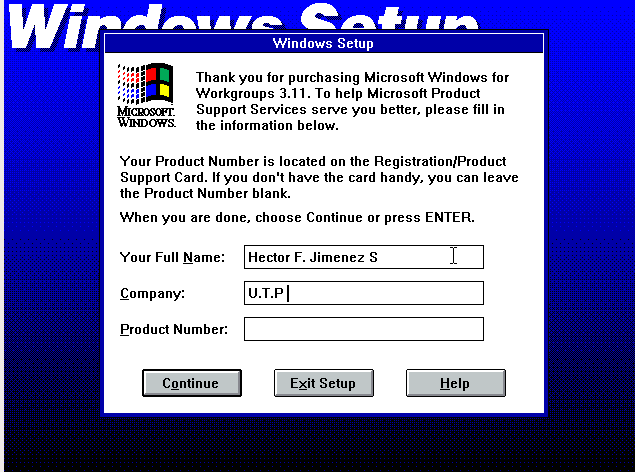
\includegraphics[width=0.68\textwidth]{img/2.png}
        }}
        \subfloat[Verificacion de información, Windows3.11 setup]{\label{fig:sugerencia}{
   		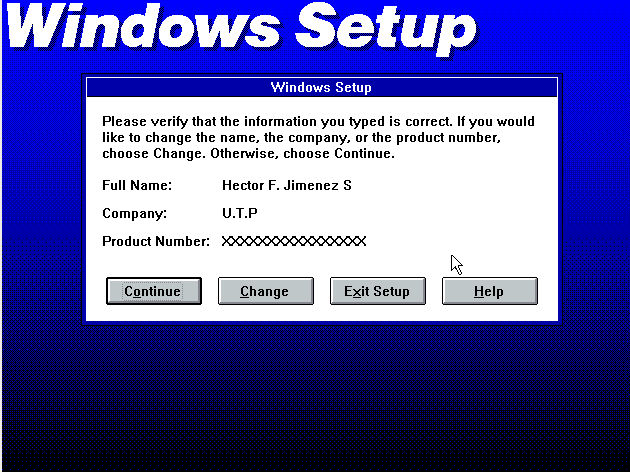
\includegraphics[width=0.68\textwidth]{img/3.png}
        }}
        \hfill
        \subfloat[Seleccion de Componentes, Windows3.11 setup]{\label{fig:disponibles}{
   		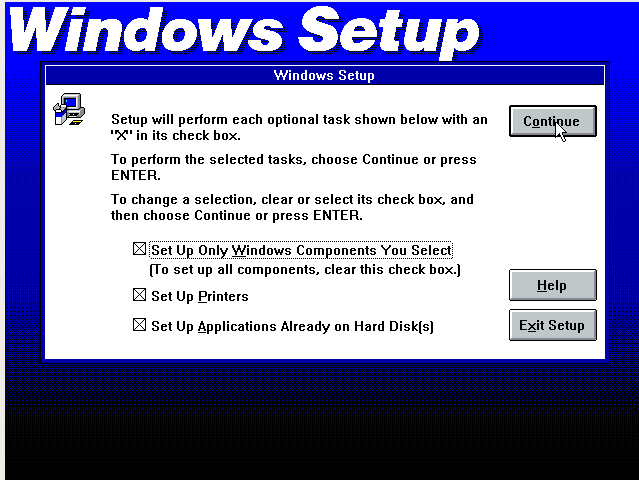
\includegraphics[width=0.68\textwidth]{img/4.png}
        }}
        \subfloat[Solicitud Ingreso disco 3 instalador Windows3.11 setup ]{\label{fig:sugerencia}{
   		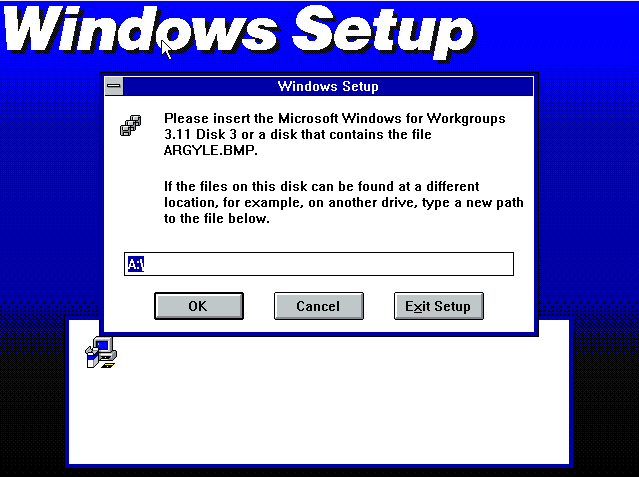
\includegraphics[width=0.68\textwidth]{img/5.png}
        }}
        \hfill
        \subfloat[Solicitud Ingreso disco 4 instalador Windows3.11 setup ]{\label{fig:disponibles}{
   		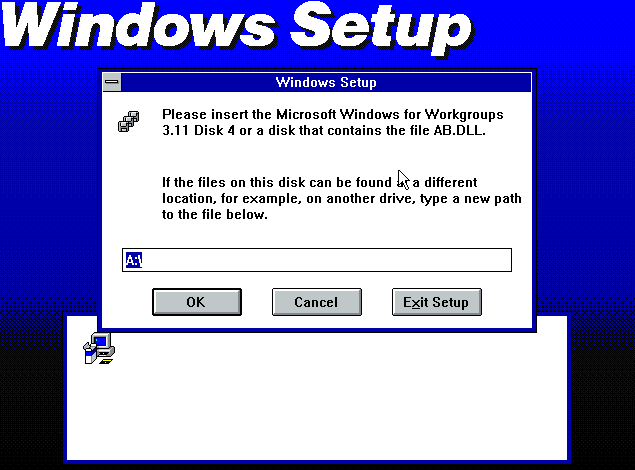
\includegraphics[width=0.68\textwidth]{img/6.png}
        }}
        \subfloat[Configuraciones de Red]{\label{fig:disponibles}{
   		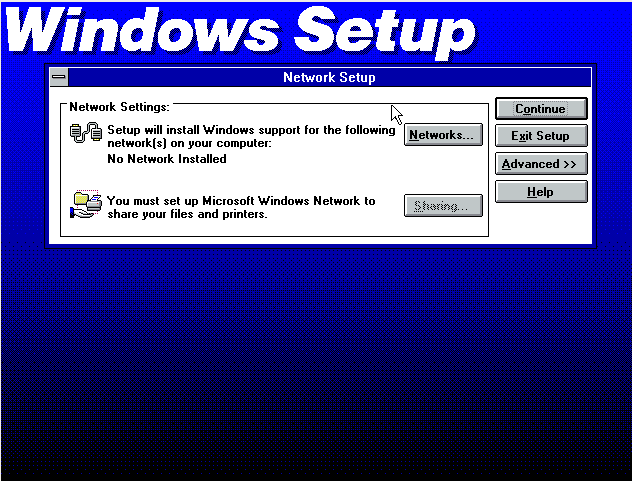
\includegraphics[width=0.68\textwidth]{img/8.png}
        }}
	\caption{Instalación de Windows3.11, Pasos Específicos.}
\end{figure}

\begin{figure}[H]
 	\centering
	\subfloat[Paso Inicial de Configuración de red Windows3.11 setup]{\label{fig:red1}{
   		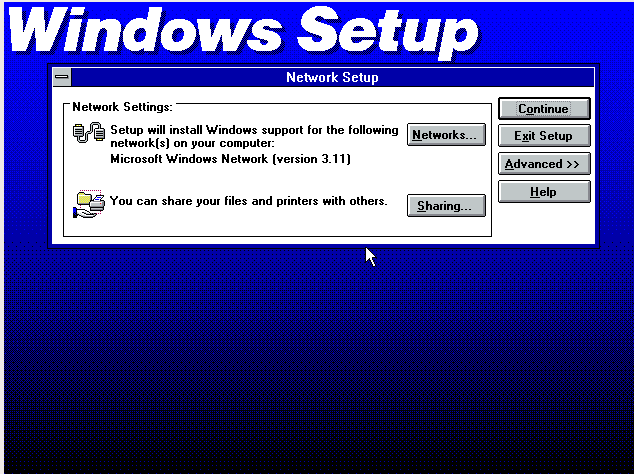
\includegraphics[width=0.68\textwidth]{img/9.png}
        }}
        \subfloat[Identificacion del grupo de trabajo]{\label{fig:sugerencia}{
   	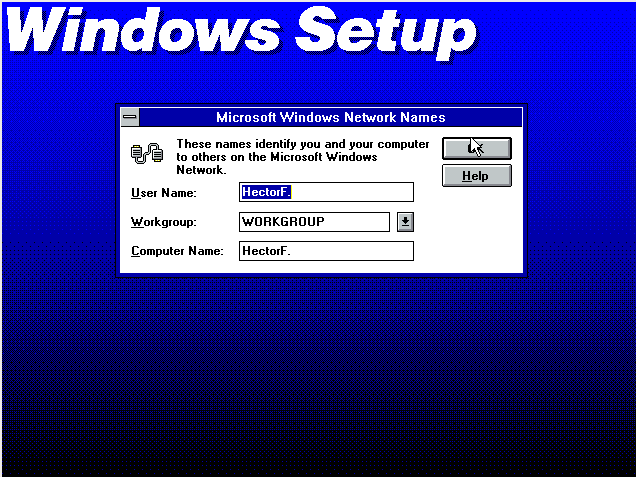
\includegraphics[width=0.68\textwidth]{img/10.png}
        }}
        \hfill
        \subfloat[Finalizacion de Instalación Windows3.11]{\label{fig:disponibles}{
   		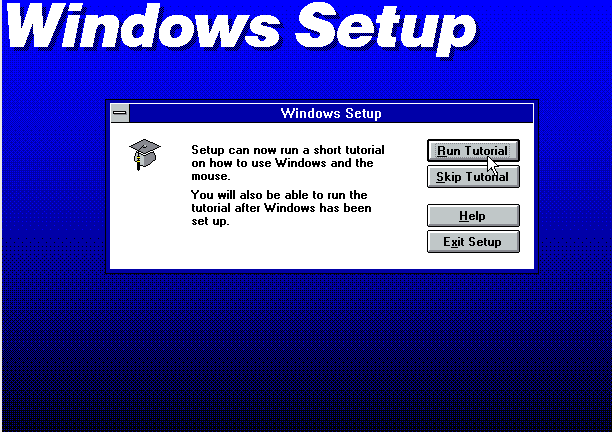
\includegraphics[width=0.68\textwidth]{img/11.png}
        }}
        \subfloat[Tutorial de Bienvenida]{\label{fig:sugerencia}{
   		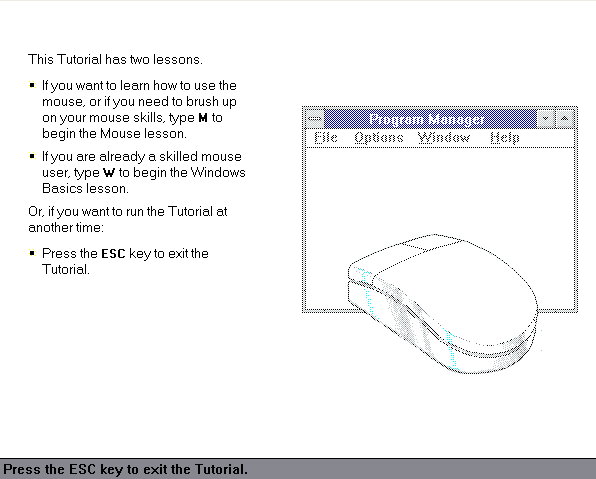
\includegraphics[width=0.68\textwidth]{img/12.png}
        }}
        \hfill
        \subfloat[Explicacion Administración de Programas]{\label{fig:disponibles}{
   		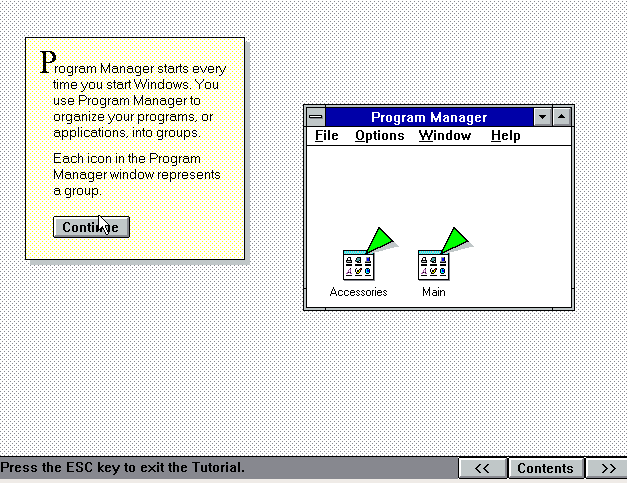
\includegraphics[width=0.68\textwidth]{img/13.png}
        }}
        \subfloat[Administracion de Programas]{\label{fig:disponibles}{
   		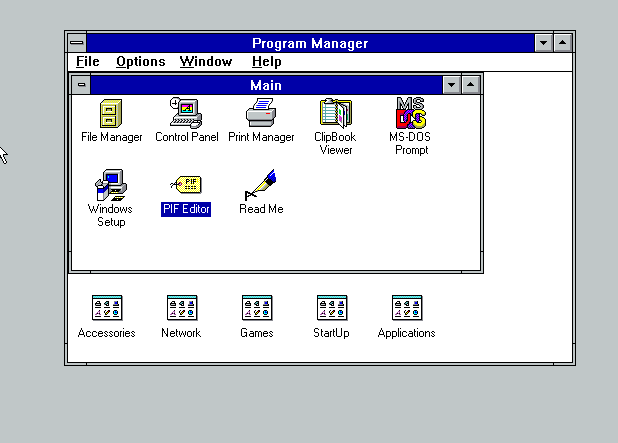
\includegraphics[width=0.68\textwidth]{img/14.png}
        }}
	\caption{Instalación de Windows3.11, Pasos Específicos, finalizados.}
\end{figure}


\begin{figure}[H]
 	\centering
	\subfloat[Verificacion de Hora y Fecha,obtenida de BIOS sistema]{\label{fig:red1}{
   		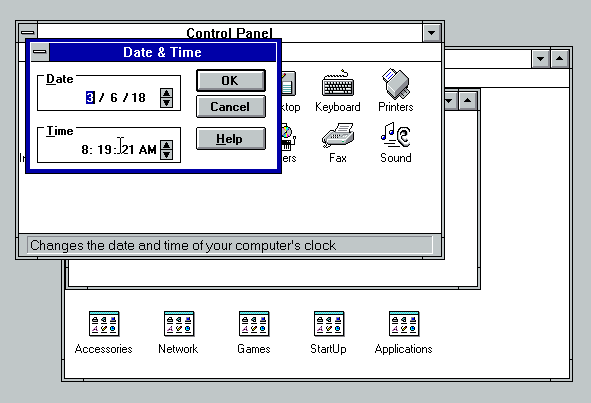
\includegraphics[width=0.68\textwidth]{img/15.png}
        }}
        \subfloat[Configuracion de Video, Pantalla]{\label{fig:sugerencia}{
   	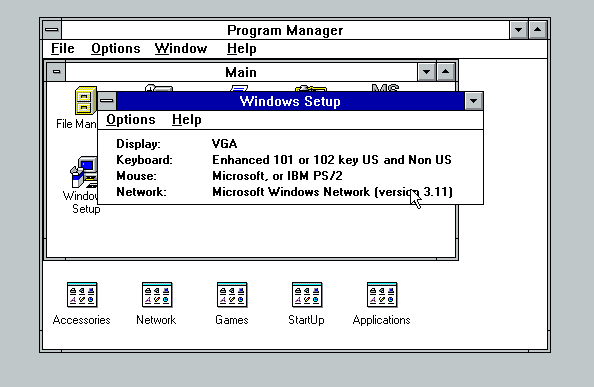
\includegraphics[width=0.68\textwidth]{img/16.png}
        }}
	\caption{Algunas opciones de los menús gráficos Windows.}
\end{figure}
\section{Instalación de  Aplicaciones}
Para realizar esta sección se realizo la instalación del programa ofimática provisto por el docente, la instalación de software para ese tiempo tal cual como se hace hoy en día incluye ejecutar \textbf{\textit{SETUP.EXE}}, es claro que la instalación de programas se encuentran en  disquetes. Con la venta comercial del procesador de textos y suite ofimática Word6.0 en 1993 Microsoft gano un terreno privilegia combatiendo con otros productos similares para otros parecidos. 


Word6.0 introdujo algunas caracteristicas interesantes como el corrector ortográfico, autoformato para una gran cantidad de texto. 

La instalación  de word6.0 puede ser observada en las figuras siguientes : 


\begin{figure}[H]
 	\centering
	\subfloat[Instalacion inicial]{\label{fig:red1}{
   		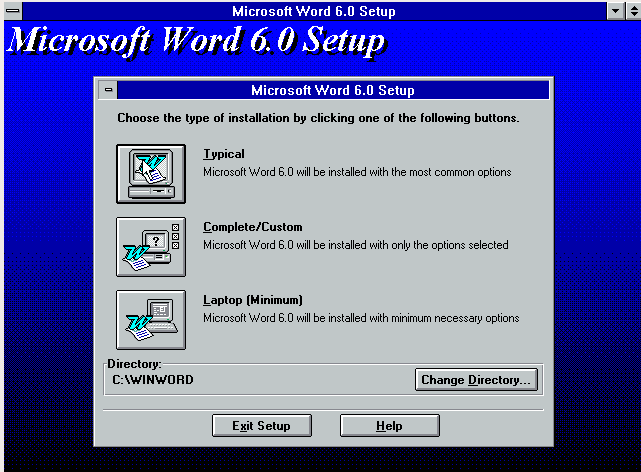
\includegraphics[width=0.68\textwidth]{img/17.png}
        }}
        \subfloat[ingreso de disquete 2]{\label{fig:sugerencia}{
   	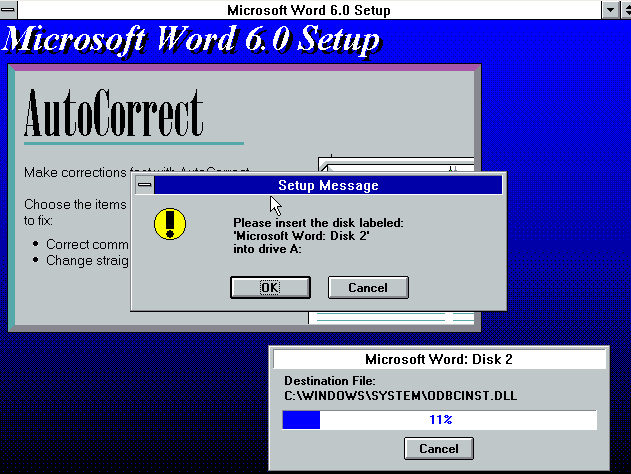
\includegraphics[width=0.68\textwidth]{img/18.png}
        }}
        \hfill
        \subfloat[ingreso de disquete 3]{\label{fig:disponibles}{
   		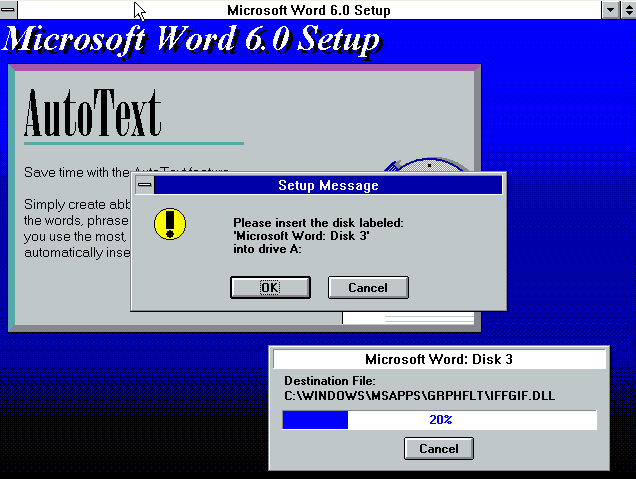
\includegraphics[width=0.68\textwidth]{img/19.png}
        }}
        \subfloat[ingreso de disquete 8]{\label{fig:sugerencia}{
   		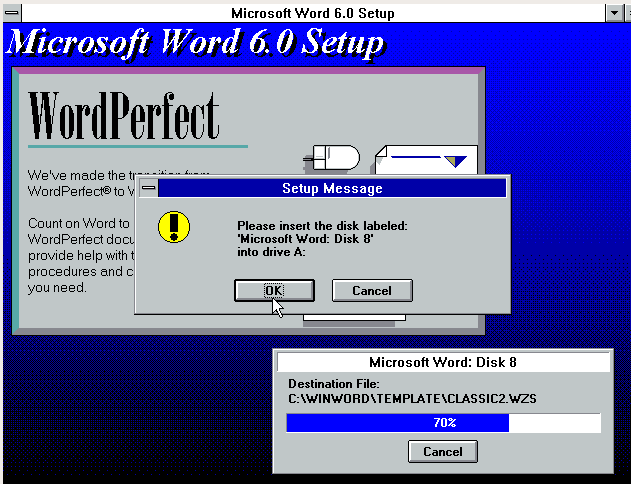
\includegraphics[width=0.68\textwidth]{img/21.png}
        }}
        \hfill
        \subfloat[Finalizacion de instalación de Word6.0]{\label{fig:disponibles}{
   		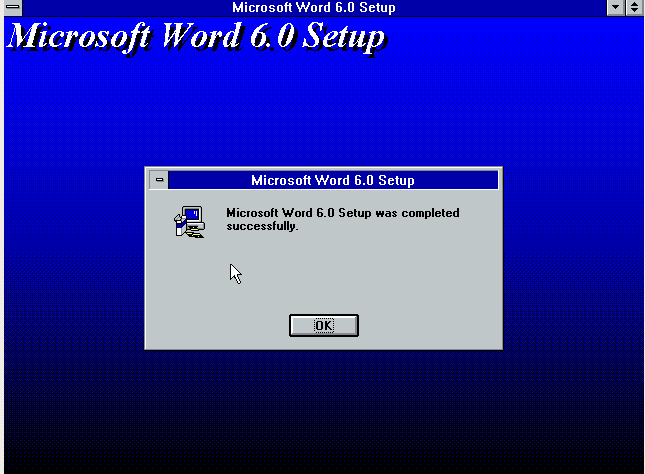
\includegraphics[width=0.68\textwidth]{img/22.png}
        }}
        \subfloat[Paquetes instalados con la instalación]{\label{fig:disponibles}{
   		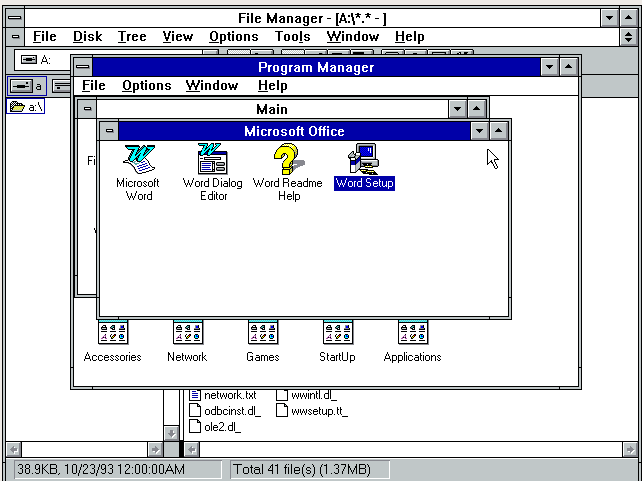
\includegraphics[width=0.68\textwidth]{img/23.png}
        }}
	\caption{Instalación de Windows3.11, Pasos Específicos, finalizados.}
\end{figure}
\section{Notas}
La gestión de archivos, se realizaba de la misma forma como se realiza en Windows6.22, como se ha mencionado la actualización mas significativa fue la incorporación de drivers de red de diferentes fabricantes, y las posibilidades de implementar workgroups para el manejo de mensajes de red usando el protocolo SMB.
\section{Referencias}
\begin{itemize}
\item  \hyperref[http://www.instructables.com/id/How-To-Install-DOS-622-Under-VirtualBox/]{DOS Manual Installation,soluciona el error de vídeo,  http://www.instructables.com/id/How-To-Install-DOS-622-Under-VirtualBox/}
\item  \hyperref[https://en.wikipedia.org/wiki/History_of_Microsoft_Word]{History of Microsoft Word, https://en.wikipedia.org/wiki/History-of-Microsoft-Word  }
\end{itemize}
\end{document}